\section{\texttt{GraviDy}}

%\begin{frame}
%    \begin{center}
%        {\Huge \texttt{GraviDy}}
%    \end{center}
%\end{frame}

\begin{frame}
    \frametitle{\texttt{GraviDy}}
    \framesubtitle{Introduction}
    \begin{center}
        \blue{\texttt{GraviDy}} is a semi-Keplerian $N$-body integrator based on heterogeneous computing.
    \end{center}
    \vspace{1cm}
    \small
    {
    \begin{block}{Heterogeneous computing}
            ``A system that use a variety of different types of computational units.''
    \end{block}
    }
\end{frame}

\begin{frame}
    \frametitle{\texttt{GraviDy}}
    \framesubtitle{Introduction}
    \begin{itemize}
        \item $N$-body problem.
        \begin{itemize}
            \item \emph{``Predicting motion of a group or celestial objects that interact each other gravitationally''.}
            \item Mostly used to work with \blue{globular clusters} (only bodies with similar masses!)
            \item The bodies are represented as a \blue{point} with mass.
            \item More than 50 years on the development of new ideas and schemes.
        \end{itemize}
    \end{itemize}
\end{frame}


\begin{frame}
    \frametitle{\texttt{GraviDy}}
    \framesubtitle{Introduction}

    Why GPU Computing?

    \begin{itemize}
        \item<2-> The $N$-body problem (collisionless) is one of the most common examples
                  to explain the utility of the GPU Computing.
        \begin{itemize}
            \item<3-> NVIDIA CUDA SDK includes an example.
        \end{itemize}
    \end{itemize}
\end{frame}


\begin{frame}
    \frametitle{\texttt{GraviDy}}
    \framesubtitle{Introduction}

    Is this a good reason to use it?

    \begin{itemize}
        \item<2-> Beware of the lies!
        \begin{itemize}
            \item<2-> It is \red{NOT} true that the GPU Computing is the solution
                      for everything.
        \end{itemize}
    \end{itemize}
\end{frame}

\begin{frame}
    \frametitle{\texttt{GraviDy}}
    \framesubtitle{Introduction}

    Is this a good reason to use it?

    \begin{itemize}
        \item<1-> GPU Computing is presented as a good solution in a lot of publications
                 related to $N$-body integrators.
        \begin{itemize}
            \item<2-> \emph{High Performance massively parallel direct $N$-body simulation on
                      large GPU Clusters}
                      (\blue{Berczik et al.}~\cite{berczik2011high}), 2011.
            \item<3-> \emph{Accelerating NBODY6 with Graphics Processing Units}
                      (\blue{Nitadori and Aarseth}~\cite{2012MNRAS.424..545N}), 2012.
            \item<4-> \emph{A fully parallel, high precision, N-body code running on hybrid
                      computing platforms}
                      (\blue{Capuzzo-Dolcetta et al.}~\cite{2012arXiv1207.2367C}), 2012.
        \end{itemize}
    \end{itemize}
\end{frame}

\begin{frame}
    \frametitle{\texttt{GraviDy}}
    \framesubtitle{Features}
    \begin{itemize}
        \item Based on a 4th order Hermite integrator (Predictor-Corrector).
        \item Using block-timesteps for the particles.
        \item Includes a special treatment to work with the massive central object (\blue{On development}).
    \end{itemize}
\end{frame}

\begin{frame}
    \frametitle{GraviDy}
    \framesubtitle{Predictor-Corrector procedure (Hermite 4th order)}
    \begin{enumerate}
        \item Initial $a$ and $a^{(1)}$ calculation.
        \item Initial block timesteps calculation.
        \item Select particles to move.
        \begin{enumerate}
            \item Calculate the predicted position and velocity.
            \item Calculate the $a$, $a^{(1)}$, $a^{(2)}$ and $a^{(3)}$.
            \item Apply the correction to the position and velocity.
            \item Update timesteps.
        \end{enumerate}
    \end{enumerate}
\end{frame}



\begin{frame}
    \frametitle{\texttt{GraviDy}}
    \framesubtitle{Features}
    Why an special treatment to work with a massive central object?
    \begin{figure}
        \centering
        \label{fig:energy}
        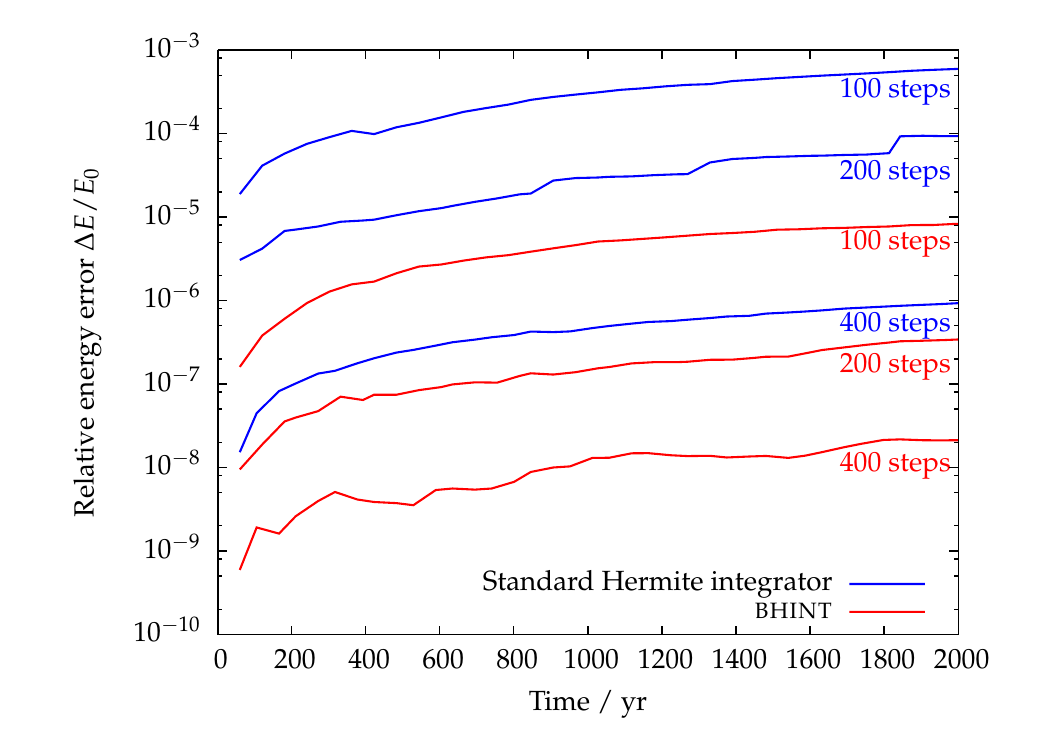
\includegraphics[width=0.7\textwidth]{img/bhint_errors}
        \caption{BHINT \blue{Loeckmann and Baumgardt}~\cite{2006IAUJD...6E..24L}}
    \end{figure}
\end{frame}


\begin{frame}
    \frametitle{\texttt{GraviDy}}
    \framesubtitle{Code}
    \begin{columns}
        \begin{column}{0.5\textwidth}
            \begin{itemize}
                \item Written in C++ and CUDA.
                \item Modular developing.
            \end{itemize}
        \end{column}
        \begin{column}{0.5\textwidth}
            \begin{figure}
                \centering
                \label{fig:navaja}
                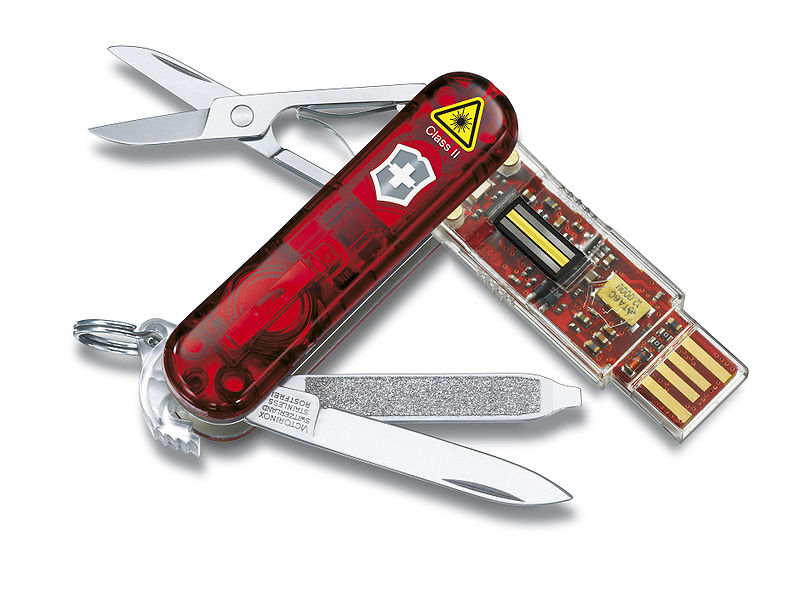
\includegraphics[width=0.8\textwidth]{img/navaja}
                %\caption{}
            \end{figure}
        \end{column}
    \end{columns}
    \begin{center}
        \small{
        \emph{``Always code as if the person who will maintain your code is a
        maniac serial killer that knows where you live''.}
        }
    \end{center}
\end{frame}

%\begin{frame}
%    \frametitle{\texttt{GraviDy}}
%    \framesubtitle{Predictor-Corrector procedure (Hermite 4th order)}
%    \begin{enumerate}
%        \item Initial $a$ and $a^{(1)}$ calculation.
%        \item Initial block timesteps calculation.
%        \item Select particles to move.
%        \begin{enumerate}
%            \item Calculate the predicted position and velocity.
%            \item Calculate the $a$, $a^{(1)}$, $a^{(2)}$ and $a^{(3)}$.
%            \item Apply the correction to the position and velocity.
%            \item Update timesteps.
%        \end{enumerate}
%    \end{enumerate}
%\end{frame}

\begin{frame}[fragile]
    \frametitle{\texttt{GraviDy}}
    \framesubtitle{Keplerian correction}

    \begin{eqnarray}
        \boldsymbol{a}_{i} = \sum\limits_{\substack{j=0\\j\neq i}}^{N} G m_{j} \dfrac{\boldsymbol{r}_{ij}}{r_{ij}^{3}}
    \end{eqnarray}


    Based on the main idea behind the integrator developed by \blue{Loeckmann and Baumgardt}~\cite{2006IAUJD...6E..24L}.
    \begin{eqnarray}
        \boldsymbol{a}_{i} =   \underbrace{ - G m_{0}
                                          \dfrac{\boldsymbol{r}_{i}}{r_{i}^{3}}
                                          }_{unperturbed\ motion}
                             - \underbrace{ \sum\limits_{\substack{j=1\\j\neq i}}^{N-1}
                                            G m_{j} \dfrac{\boldsymbol{r}_{ij}}{r_{ij}^{3}}
                                          }_{perturbing\ force}
    \end{eqnarray}
\end{frame}

\begin{frame}
    \frametitle{\texttt{GraviDy}}
    \framesubtitle{Kepler's correction}
    \begin{enumerate}
        \item New position of a particle after a time step $\Delta t$:
        \begin{eqnarray}
            \boldsymbol{r'} =    \boldsymbol{      r}              +
                                       \boldsymbol{      v} \Delta t     &+&
                         \dfrac{1}{2!} \boldsymbol{      a}_{K} \Delta t^{2} +
                         \dfrac{1}{3!} \boldsymbol{\dot{a}}_{K} \Delta t^{3} + \ldots \nonumber\\
                          &+& 
                         \dfrac{1}{2!} \boldsymbol{      a}_{P} \Delta t^{2} +
                         \dfrac{1}{3!} \boldsymbol{\dot{a}}_{P} \Delta t^{3} + \ldots
        \end{eqnarray}
        \item With Kepler's correction:
        \begin{eqnarray}
            \boldsymbol{r}_{pred} =    \blue{\boldsymbol{      r}_{k,pred}}         +
                         \dfrac{1}{2!}       \boldsymbol{      a}_{i} \Delta t^{2} +
                         \dfrac{1}{3!}       \boldsymbol{\dot{a}}_{i} \Delta t^{3} \\
            \boldsymbol{v}_{pred} =    \blue{\boldsymbol{      v}_{k,pred}}         +
                         \dfrac{1}{2!}       \boldsymbol{      a}_{i} \Delta t^{2} +
                         \dfrac{1}{3!}       \boldsymbol{\dot{a}}_{i} \Delta t^{3}
        \end{eqnarray}

    \end{enumerate}
\end{frame}

\begin{frame}
    \frametitle{Preliminary results (performed @ AEI)}
    \framesubtitle{Hardware}
    \begin{description}
        \item[GPU]
            Nvidia Tesla C2050 @ 1.5GHz (448 cores)
        \item[CPU]
            Intel Xeon CPU E5504  @ 2.00GHz (4 cores)
    \end{description}
\end{frame}

%\begin{frame}
%    \frametitle{Preliminary results}
%    \framesubtitle{Energy Errors (Relative and Absolute)}
%    \begin{itemize}
%        \item CPU:  \sim $10^{-13} - \sim 10^{-16}$
%        \item GPU:  \sim $10^{-12} - \sim 10^{-15}$
%    \end{itemize}
    %\begin{tabular}{l|r|r|r|r}
    %    Error    & 1024 & 2048 & 4096 & 8192 \\
    %    Relative CPU& \~10^{-14} & \~10^{-14}
    %    Relative GPU& 
    %    Absolute CPU& \~10^{-14}
    %    Absolute GPU&
    %\end{tabular}
    %\begin{figure}
    %    \centering
    %    \label{fig:init-time}
    %    %\includegraphics[width=0.8\textwidth]{img/result-init_accjerk}
    %    \caption{Energy Conservation}
    %\end{figure}
%\end{frame}

\begin{frame}
    \frametitle{Preliminary results}
    \begin{figure}
        \centering
        \label{fig:init}
        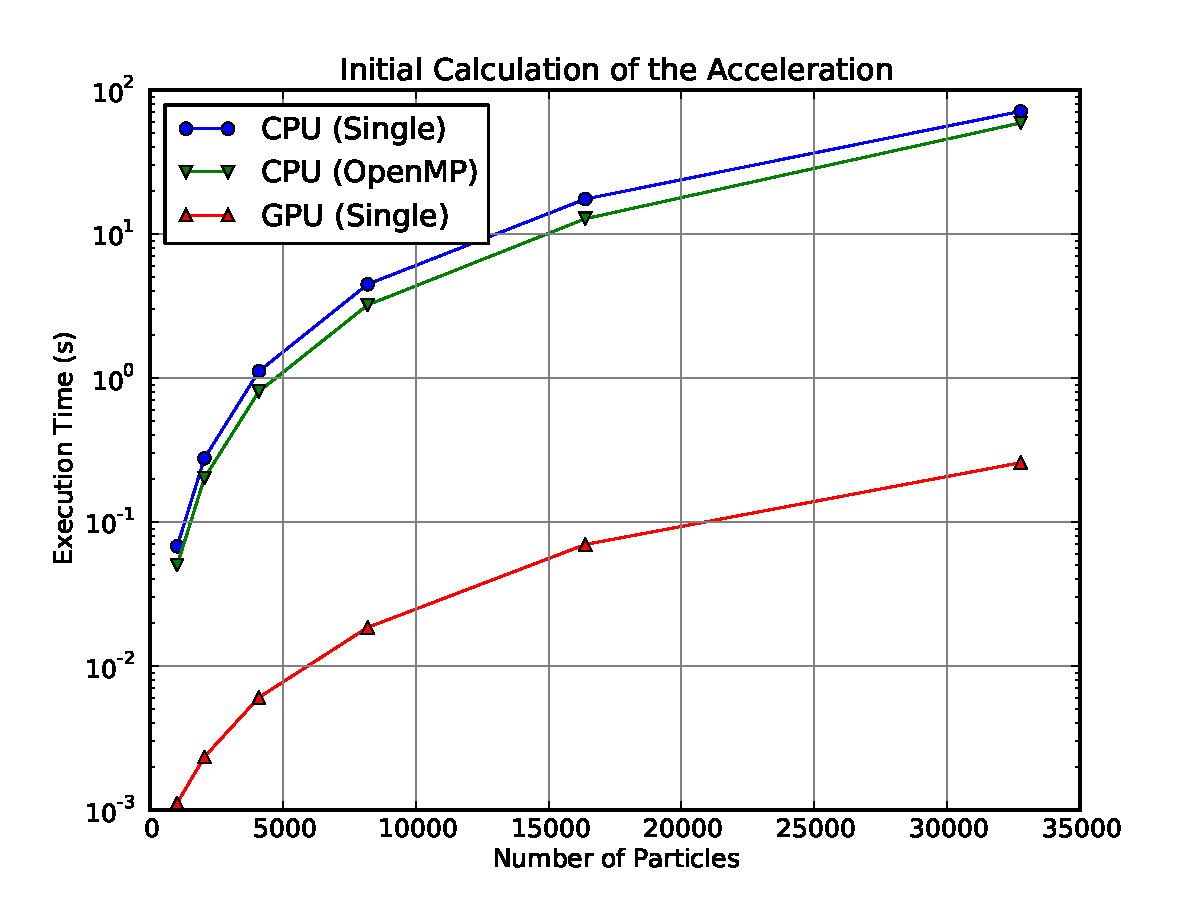
\includegraphics[width=0.7\textwidth]{img/init}
        %\caption{Acceleration calculation}
    \end{figure}
\end{frame}

\begin{frame}
    \frametitle{Preliminary results}
    \begin{figure}
        \centering
        \label{fig:energy}
        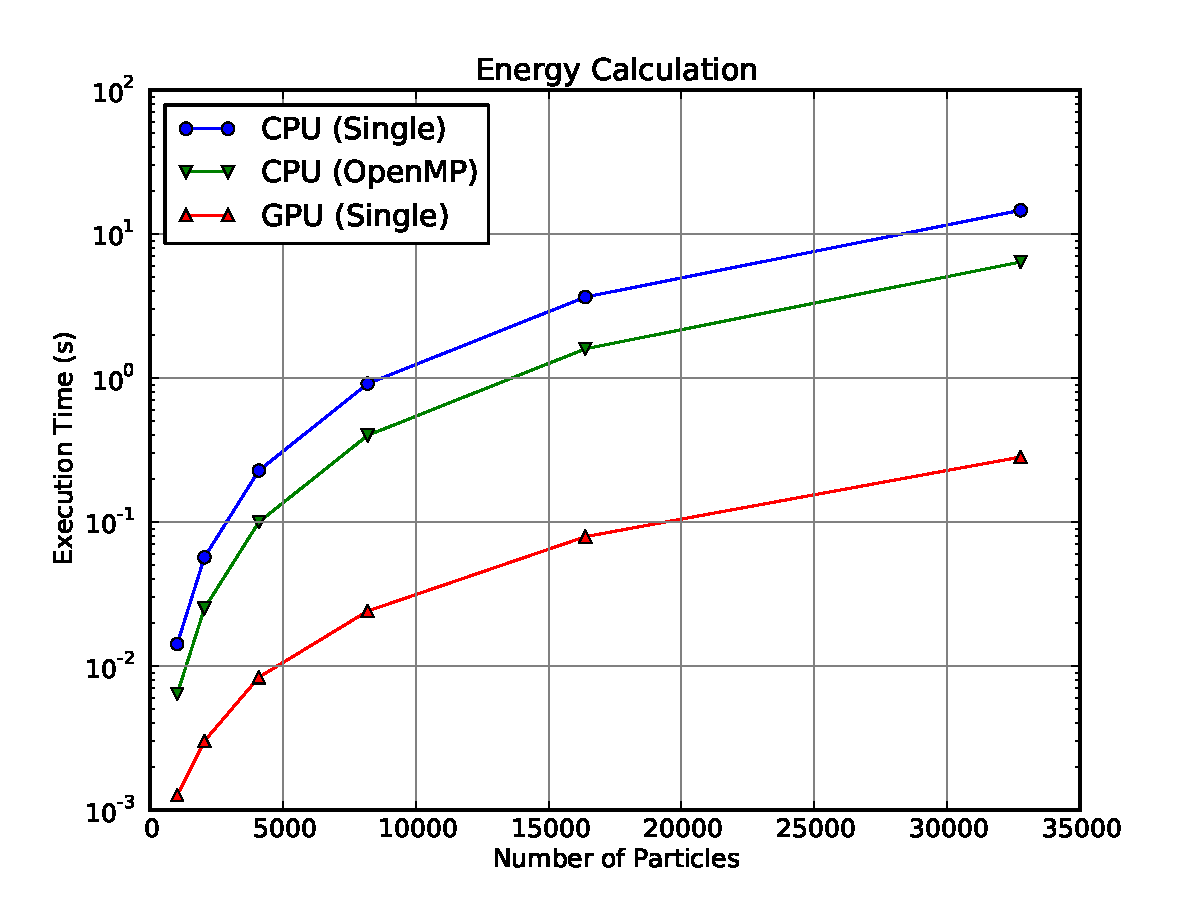
\includegraphics[width=0.7\textwidth]{img/energy.pdf}
        %\caption{Energy calculation}
    \end{figure}
\end{frame}


\begin{frame}[fragile]
    \frametitle{Preliminary results}
    \framesubtitle{The amount of work dilemma}

    \begin{lstlisting}
        init_acc_jerk();
        while (ITIME < int_time)
        {
            total = find_particles_to_move();
            predicted_pos_vel();
            update_acc_jerk(total); // Only a few particles!
            correction_pos_vel(total);
        }
    \end{lstlisting}
\end{frame}

\begin{frame}[fragile]
    \frametitle{Preliminary results}
    \framesubtitle{The amount of work dilemma}

    At the beginning of the integration:

    \begin{lstlisting}
        void init_acc_jerk()
        {
            for (int i = 0; i < N; i++)
                for (int j = 0; j < N; j++)
                    force_interation(i, j);
        }
    \end{lstlisting}

    In each integration step:

    \begin{lstlisting}
        void update_acc_jerk()
        {
            for (int i = 0; i < total; i++) // total < N (~ 10%)
                for (int j = 0; j < N; j++)
                    force_interation(i, j);
        }
    \end{lstlisting}
\end{frame}

\begin{frame}[fragile]
    \frametitle{Preliminary results}
    \framesubtitle{The amount of work dilemma}

    Is that enough?

    \texttt{gprof} tell us that is \red{not} enough.
    \tiny{
    \begin{lstlisting}
time  seconds  seconds      calls s/call s/call  name
80.46    87.52   87.52 1296647743   0.00   0.00  force_calculation(int, int)
11.44    99.96   12.44     799495   0.00   0.00  init_dt(float*)
 3.41   103.67    3.71     414230   0.00   0.00  save_old()
 3.04   106.98    3.31     414230   0.00   0.00  correction_pos_vel(float, int)
 0.96   108.02    1.04     414230   0.00   0.00  find_particles_to_move(float)
 0.70   108.78    0.76     414230   0.00   0.00  next_itime(float*)
 0.00   108.78    0.00     414230   0.00   0.00  get_energy_log(int, float)
 0.00   108.78    0.00     414230   0.00   0.00  update_acc_jrk(int)
 0.00   108.78    0.00     414230   0.00   0.00  predicted_pos_vel(float)
 0.00   108.78    0.00       2048   0.00   0.00  magnitude(double, double, double)
    \end{lstlisting}
    }

\end{frame}


\begin{frame}[fragile]
    \frametitle{Preliminary results}
    \framesubtitle{The amount of work dilemma}

    The amount of thread that we can run in parallel is \red{$21,504$}.

    \begin{itemize}
        \item<2-> We need to define a strategy to use all the GPU capability.
        \begin{itemize}
            \item<3-> Not easy.
            \item<3-> Most of the really-simple ideas degrade the performance.
        \end{itemize}
        \item<4-> Be careful of:
        \begin{itemize}
            \item<5-> The amount of data that you will copy between CPU and GPU.
            \item<5-> Synchronization of the threads.
            \item<5-> GPU memory access.
            \item<5-> etc.
        \end{itemize}
    \end{itemize}
\end{frame}
